\documentclass[64pt,aspectratio=169]{beamer}

\usetheme{mpiisimple}

\usepackage{soul}
\usepackage{pdfcomment}
\usepackage[utf8]{inputenc}
\usepackage{graphicx}
\usepackage{amsmath,amsfonts,amssymb,amsthm}
\usepackage{xspace}
\usepackage{xcolor}
\usepackage{tabularx}
\usepackage{multirow}
\usepackage{nicefrac}
\usepackage{pgfplots}
\usepackage[skins]{tcolorbox}
\usepackage{tikz}
\usetikzlibrary{calc}
\usetikzlibrary{math}
\usetikzlibrary{fadings}
\usetikzlibrary{arrows.new}
\newcommand*\circled[1]{\tikz[baseline=(char.base)]{
		\node[shape=circle,draw=MPIIorange,fill=MPIIorange,inner sep=2pt] (char) {\color{MPIIwhite}#1};}}
\tikzset{arrow/.style={-latex new,arrow head=0.25cm}}
\definecolor{colorbrewer0}{RGB}{45,45,45}
\definecolor{colorbrewer1}{RGB}{228,26,28}
\definecolor{colorbrewer2}{RGB}{55,126,184}
\definecolor{colorbrewer3}{RGB}{77,175,74}
\definecolor{colorbrewer4}{RGB}{152,78,163}
\definecolor{colorbrewer5}{RGB}{255,127,0}
\definecolor{colorbrewer6}{RGB}{255,255,51}
\definecolor{colorbrewer7}{RGB}{166,86,40}
\definecolor{colorbrewer8}{RGB}{247,129,191}
\definecolor{colorbrewer9}{RGB}{153,153,153}
\definecolor{colorbrewer10}{RGB}{24,167,181}

\usepackage{tcolorbox}\usepackage{tcolorbox}
\tcbuselibrary{skins,breakable}

\newenvironment{paper}[1]{%
    \tcolorbox[noparskip,frame hidden,boxrule=0.5mm,colframe=gray,
    colback=gray!25!white,coltext=MPIIblack,
    sharpish corners,no shadow,
    left=1.5mm,top=1.5mm,right=1.5mm,bottom=1mm,]}%
{\endtcolorbox}
\tcbuselibrary{skins,breakable}
	
\definecolor{colorbrewer1}{RGB}{228,26,28}
\definecolor{colorbrewer2}{RGB}{55,126,184}
\definecolor{colorbrewer3}{RGB}{77,175,74}
\definecolor{colorbrewer4}{RGB}{152,78,163}
\definecolor{colorbrewer5}{RGB}{255,127,0}
\definecolor{colorbrewer6}{RGB}{255,255,51}
\definecolor{colorbrewer7}{RGB}{166,86,40}
\definecolor{colorbrewer8}{RGB}{247,129,191}
\definecolor{colorbrewer9}{RGB}{153,153,153}

\DeclareMathOperator*{\argmax}{argmax~}
\DeclareMathOperator*{\argmin}{argmin~}
\DeclareMathOperator{\sign}{sign}
\DeclareMathOperator*{\ntimes}{\!\times\!}
\newcommand{\Id}{\mathbbm{1}}
\DeclareRobustCommand{\RTE}{%
	\ifmmode
	\text{RErr}
	\else
	RErr\xspace
	\fi
}

\makeatletter
\DeclareRobustCommand\onedot{\futurelet\@let@token\@onedot}
\def\@onedot{\ifx\@let@token.\else.\null\fi\xspace}
\def\eg{e.g\onedot} \def\Eg{E.g\onedot}
\def\ie{i.e\onedot} \def\Ie{I.e\onedot}
\def\cf{cf\onedot} \def\Cf{Cf\onedot}
\def\etc{etc\onedot} \def\vs{vs\onedot}
\def\st{s.t\onedot}
\def\wrt{wrt\onedot}
\def\dof{d.o.f\onedot}
\def\etal{et~al\onedot} \def\iid{i.i.d\onedot}
\def\Fig{Fig\onedot} \def\Eqn{Eqn\onedot} \def\Sec{Sec\onedot} \def\Alg{Alg\onedot}
\makeatother

\author{David Stutz}
\title[Adversarial Robustness and Flat Minima]{Relating Adversarially Robust Generalization to Flat Minima}

\begin{document}
	\setbeamertemplate{footline}{
		\begin{textblock*}{\paperwidth}(4mm,82mm)
			\begin{minipage}{36mm}
				
\includegraphics[height=0.5cm]{mpilogo-inf-wide}
			\end{minipage}
			\begin{minipage}{24mm}
				
\includegraphics[height=0.525cm]{UT_WBMW_Rot_RGB}
			\end{minipage}
			\begin{minipage}{30mm}
				
\includegraphics[height=0.675cm]{Unknown-3}
			\end{minipage}
			\hfill
			\begin{minipage}{68mm}
				\raggedright\fontsize{7}{8}{\bfseries\textcolor{MPIIblack}{Adversarial Robustness and Flat Minima\ {\color{MPIIgray}--} \insertauthor}}
			\end{minipage}
			\vspace*{4mm}
		\end{textblock*}
	}
	
	\begingroup
	\setbeamertemplate{footline}{}
	\begin{frame}[plain,noframenumbering]
		\begin{center}  
			\vspace*{-0.5cm}
			\begin{minipage}[t]{4.5cm}
				\centering
				\begin{tikzpicture}
				\node at (0,0){
\includegraphics[height=1.25cm]{Unknown-3}};
				\end{tikzpicture}
			\end{minipage}
			\vspace*{-0.25cm}
						
			{\huge\bfseries Relating Adversarially Robust\\[4px] Generalization to Flat Minima}
			\vskip 0.5cm
			
			\begin{center}
				\begin{minipage}{0.225\textwidth}
					\centering
					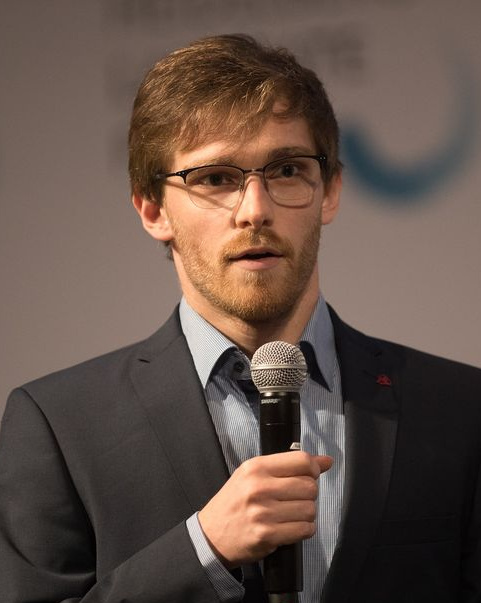
\includegraphics[height=2.5cm]{gfx/profilepicture}
						
					\footnotesize
					
					\underline{David}
					
					\underline{Stutz}
				\end{minipage}
				\begin{minipage}{0.225\textwidth}
					\centering
					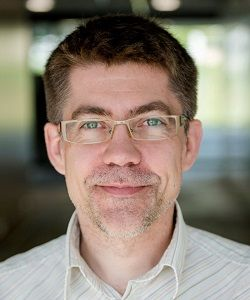
\includegraphics[height=2.5cm,trim={0.1cm 0 0.15cm 0}, clip]{gfx/matthiashein}
					
					\footnotesize
					
					Matthias
					
					Hein
				\end{minipage}
				\begin{minipage}{0.225\textwidth}
					\centering
					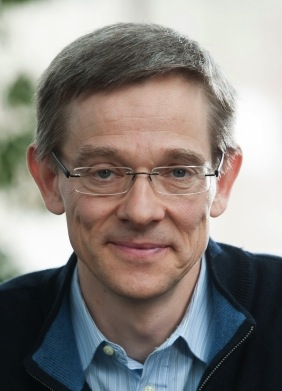
\includegraphics[height=2.5cm]{gfx/berntschiele}
					
					\footnotesize
					
					Bernt
					
					Schiele
				\end{minipage}
			\end{center}
			\vspace*{-0.25cm}
			
			\begin{minipage}[t]{4.5cm}
				\vspace*{0px}
				\centering
				\begin{tikzpicture}
				\node at (0,0){
\includegraphics[height=1.25cm]{mpilogo-inf-narrow.eps}};
				\end{tikzpicture}
			\end{minipage}
			\hspace*{0.25cm}
			\begin{minipage}[t]{4.5cm}
				\vspace*{0px}
				\centering
				\begin{tikzpicture}
				\node at (0,0){
\includegraphics[height=1.25cm]{UT_WBMW_Rot_RGB.eps}};
				\end{tikzpicture}
			\end{minipage}
		\end{center}
	\end{frame}
	\endgroup
	
	\begin{frame}[t]{\bfseries \textit{2-Minute Overview:} Robust Overfitting}
		\Large
		Adversarial training exhibits severe \emph{robust} overfitting:
		\vspace*{-2px}
		\begin{center}
			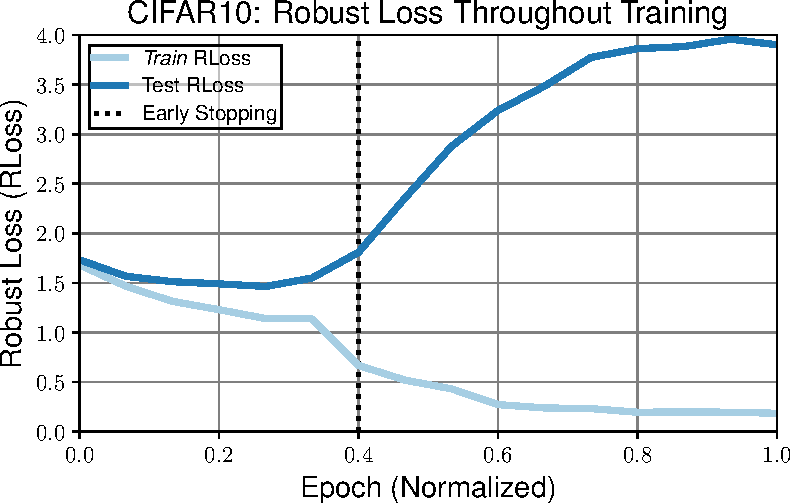
\includegraphics[height=5.5cm]{plots/talk_overview12.pdf}
		\end{center}
	\end{frame}
	
	\begin{frame}[t]{\bfseries \textit{2-Minute Overview:} Robust Flatness}
		\Large
		Robust overfitting caused by converging to \emph{sharp} minima:
		\vspace*{-2px}
		\begin{center}
			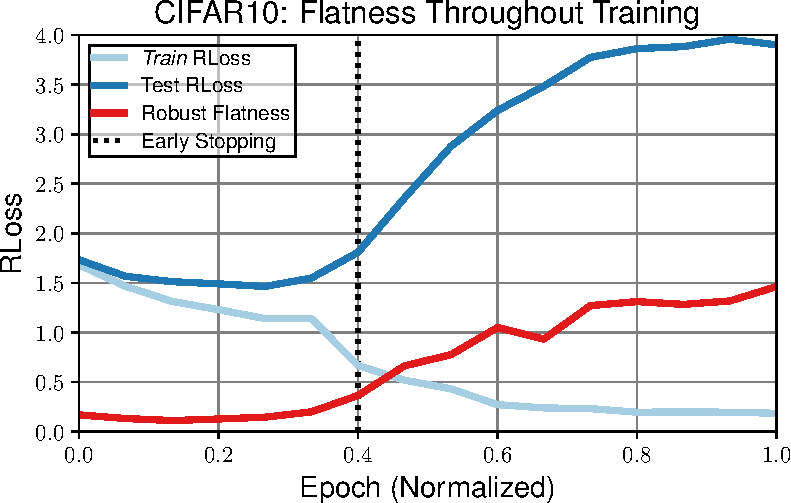
\includegraphics[height=5.5cm]{plots/talk_overview2.pdf}
		\end{center}
	\end{frame}
	
	\begin{frame}[t]{\bfseries \textit{2-Minute Overview:} Robust Flatness}
		\Large
		Robust overfitting caused by converging to \emph{sharp} minima:
		\vspace*{-2px}
		\begin{center}
			\begin{minipage}[t]{0.425\textwidth}
				\begin{tikzpicture}[remember picture]\node[opacity=0.5] at (0,0) {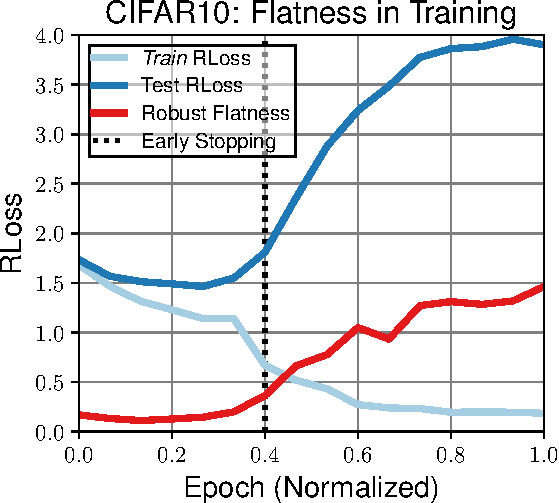
\includegraphics[height=5.5cm]{plots/talk_overview22.pdf}};\end{tikzpicture}
			\end{minipage}
			\begin{minipage}[t]{0.09\textwidth}
				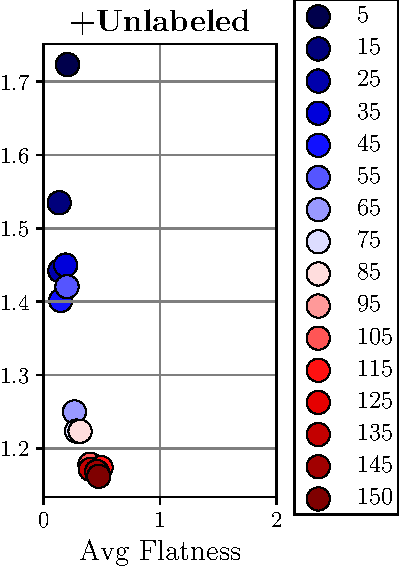
\includegraphics[height=5.5cm,clip,trim={5cm 0cm 0cm 0cm}]{../paper/plots_main_flatness_epochs_correlation_seq_500k}
			\end{minipage}
			\begin{minipage}[t]{0.275\textwidth}
				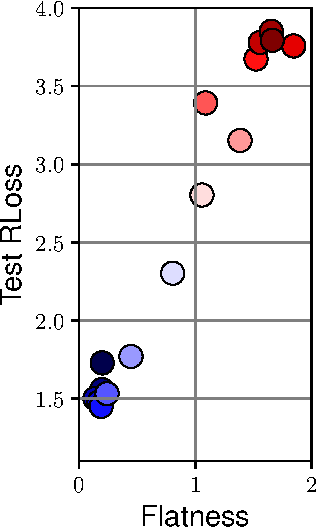
\includegraphics[height=5.5cm]{plots/talk_flatness_epochs_correlation_seq2.pdf}
			\end{minipage}
		\end{center}
	\end{frame}
	
	\begin{frame}[t]{\bfseries \textit{2-Minute Overview:} Robustness and Flatness}
		\Large
		Clear relationship between robustness and flatness:
		\vspace*{2px}
		\begin{center}
			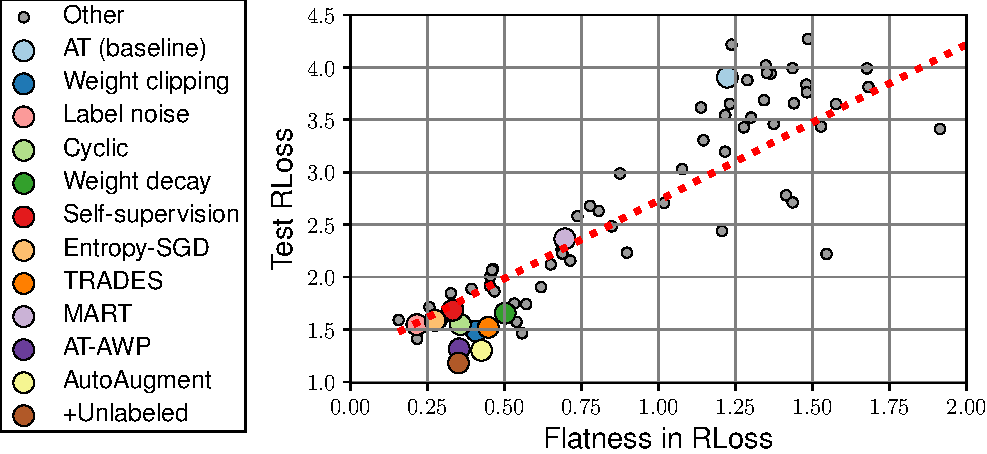
\includegraphics[height=5cm]{plots/talk_flatness_correlation_seq_loss.pdf}
		\end{center}
	\end{frame}
	
	\begin{frame}[t]{\bfseries Outline}
		\Large
		\begin{tcolorbox}[
			enhanced,
			boxsep=4pt,
			left=0pt,
			right=0pt,
			top=2pt,
			toptitle=0pt,
			bottomtitle=2pt,
			bottom=0pt,
			colback=gray!12!white,
			colframe=gray!12!white,
			width=1\textwidth, 
			enlarge left by=0mm,
			arc=0pt,outer arc=0pt,
			boxrule=1pt,
			title=,
			coltitle=MPIIblack,
			colbacktitle=gray!12!white,
			titlerule style=white,
			collower=MPIIblack,
			]
			\color{MPIIblack}
			\bfseries More details: \href{http://davidstutz.de/flatness}{\texttt{davidstutz.de/flatness}}
		\end{tcolorbox}
		
		\begin{itemize}
			\item Adversarial training and robust overfitting
			\item Hypothesis and contributions
			\item Measuring robust flatness
			\item Relationship robustness and flatness
		\end{itemize}
	\end{frame}
	
	\begin{frame}[t]{\bfseries Motivation: Adversarial Examples}
		\Large
		\vspace*{-0.25cm}
		
		\begin{center}
			\begin{tikzpicture}
				\node[anchor=north west] at (0,0){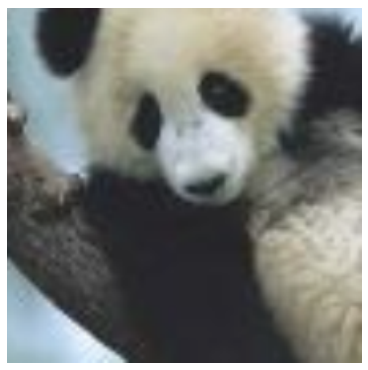
\includegraphics[width=3cm]{gfx/pandas1}};
				\node[anchor=north] at (1.6, -3.15){\small $x$};
				\node[anchor=south] at (1.6, -0.225){\small Example};
				\node[anchor=north west] at (3.5,0){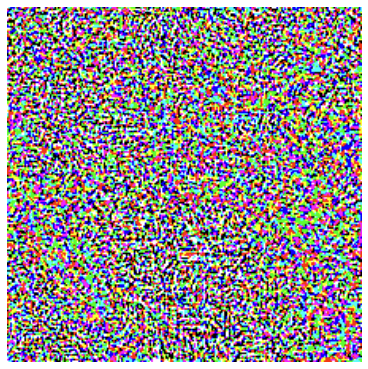
\includegraphics[width=3cm]{gfx/pandas2}};
				\node[anchor=north] at (5.1, -3.15){\small $\delta$};
				\node[anchor=south] at (5.1, -0.2){\small Adversarial Noise};
				\node[anchor=north west] at (7,0){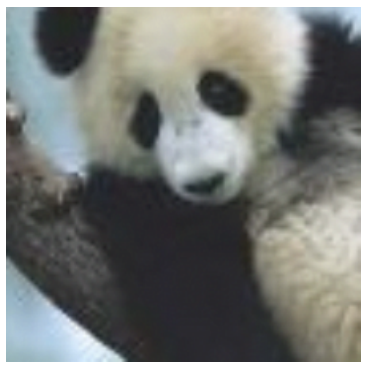
\includegraphics[width=3cm]{gfx/pandas3}};
				\node[anchor=north] at (8.6, -3.15){\small $\tilde{x}=x+\delta$};
				\node[anchor=south] at (8.6, -0.25){\small Adversarial Example};
			\end{tikzpicture}
		\end{center}
		\vspace*{-0.25cm}
		
		Adversarial examples from maximizing cross-entropy loss:
		\vspace*{-6px}
		\begin{align}
			\max_{\color{MPIIred}\|\delta\|_\infty \leq \epsilon} \mathcal{L}(f(x + \delta;w), y)\notag
		\end{align}
	\end{frame}
	
	\begin{frame}[t]{\bfseries Motivation: Adversarial Examples}
		\Large
		\vspace*{-0.25cm}
		
		\begin{center}
			\begin{tikzpicture}
				\node[anchor=north west] at (0,0){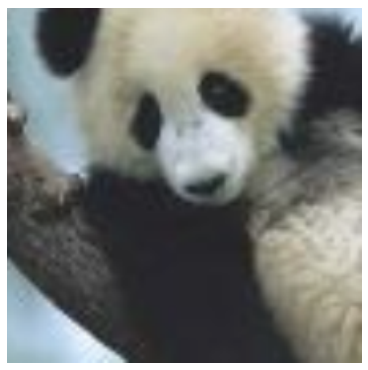
\includegraphics[width=3cm]{gfx/pandas1}};
				\node[anchor=north] at (1.6, -3.15){\small $x$};
				\node[anchor=south] at (1.6, -0.225){\small Example};
				\node[anchor=north west] at (3.5,0){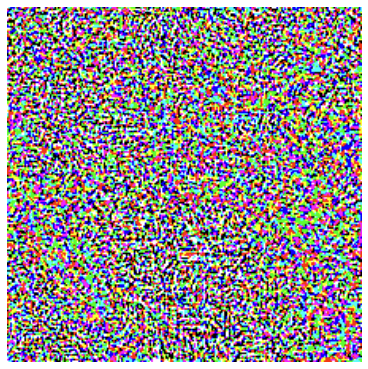
\includegraphics[width=3cm]{gfx/pandas2}};
				\node[anchor=north] at (5.1, -3.15){\small $\delta$};
				\node[anchor=south] at (5.1, -0.2){\small Adversarial Noise};
				\node[anchor=north west] at (7,0){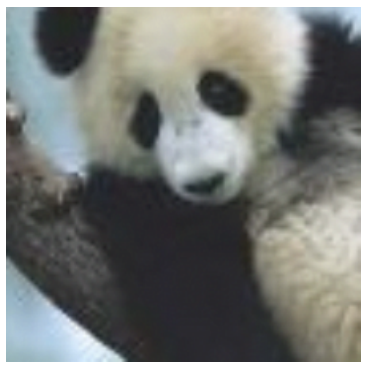
\includegraphics[width=3cm]{gfx/pandas3}};
				\node[anchor=north] at (8.6, -3.15){\small $\tilde{x}=x+\delta$};
				\node[anchor=south] at (8.6, -0.25){\small Adversarial Example};
			\end{tikzpicture}
		\end{center}
		\vspace*{-0.3cm}
		
		Adversarial examples from maximizing cross-entropy loss:
		\vspace*{-6px}
		\begin{align}
			\underbrace{\max_{\|\delta\|_\infty \leq \epsilon} \mathcal{L}(f(x + \delta;w), y)}_{\color{MPIIred} \text{\bfseries RLoss}}\notag
		\end{align}
	\end{frame}
	
	\begin{frame}[t]{\bfseries Motivation: Adversarial Training}
		\Large
		\vspace*{-0.25cm}
		
		\begin{center}
			\begin{tikzpicture}
				\node[anchor=north west] at (0,0){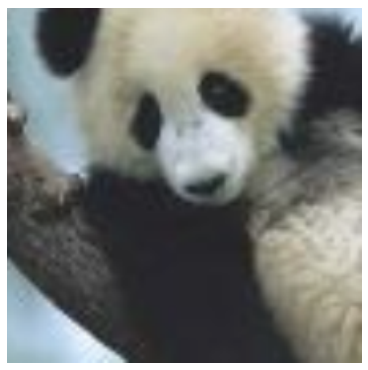
\includegraphics[width=3cm]{gfx/pandas1}};
				\node[anchor=north] at (1.6, -3.15){\small $x$};
				\node[anchor=south] at (1.6, -0.225){\small Example};
				\node[anchor=north west] at (3.5,0){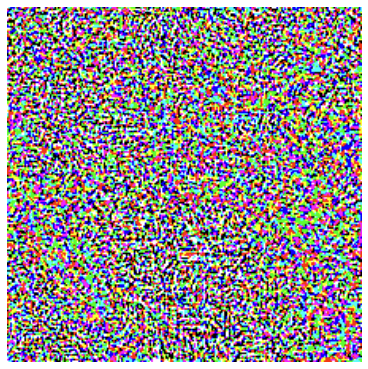
\includegraphics[width=3cm]{gfx/pandas2}};
				\node[anchor=north] at (5.1, -3.15){\small $\delta$};
				\node[anchor=south] at (5.1, -0.2){\small Adversarial Noise};
				\node[anchor=north west] at (7,0){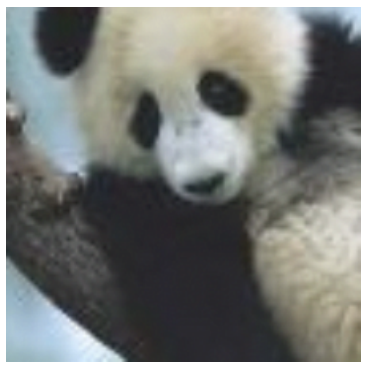
\includegraphics[width=3cm]{gfx/pandas3}};
				\node[anchor=north] at (8.6, -3.15){\small $\tilde{x}=x+\delta$};
				\node[anchor=south] at (8.6, -0.25){\small Adversarial Example};
			\end{tikzpicture}
		\end{center}
		\vspace*{-0.3cm}
		
		\emph{Adversarial training} to improve adversarial robustness:
		\vspace*{-6px}
		\begin{align}
			\min_w \mathbb{E}\left[\max_{\|\delta\|_\infty \leq \epsilon} \mathcal{L}(f(x + \delta;w), y)\right]\notag
		\end{align}
	\end{frame}
	
	\begin{frame}[t]{\bfseries Motivation: Robust Overfitting}
		\Large 
		How to avoid or improve \emph{robust} overfitting and generalization?
		
		\begin{center}
			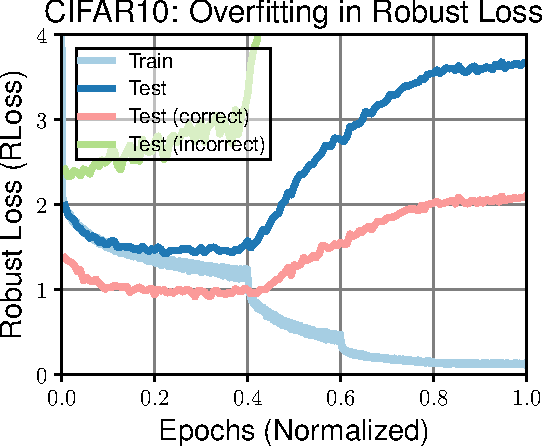
\includegraphics[height=5cm]{plots/talk_overfitting12.pdf}
		\end{center}
	\end{frame}
	
	\begin{frame}[t]{\bfseries Motivation: Robust Overfitting}
		\Large 
		How to avoid or improve \emph{robust} overfitting and generalization?
		
		\begin{center}
			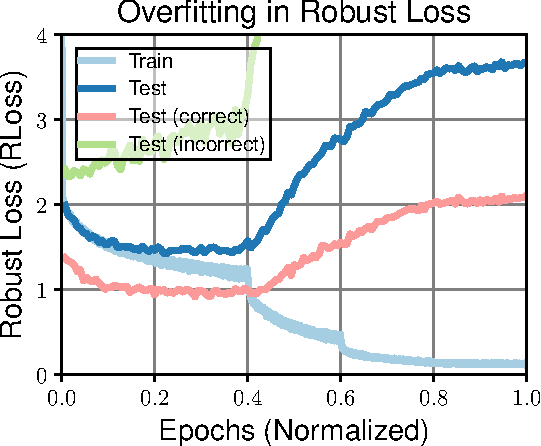
\includegraphics[height=5cm]{plots/talk_overfitting1.pdf}
			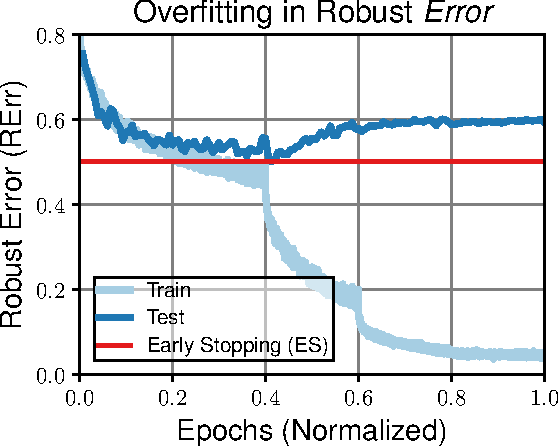
\includegraphics[height=5cm]{plots/talk_overfitting2.pdf}
		\end{center}
		\begin{tikzpicture}[remember picture,overlay]
			\node[anchor=west] at (13.5,4.65){\small 62.8\%};
			\node[anchor=west] at (13.5,4.1){\small 54.6\%};
		\end{tikzpicture}
	\end{frame}
	
	\begin{frame}[t]{\bfseries Hypothesis: Robust Flatness}
		\Large
		Flat minima in robust loss improve robust generalization:
		
		\begin{center}
			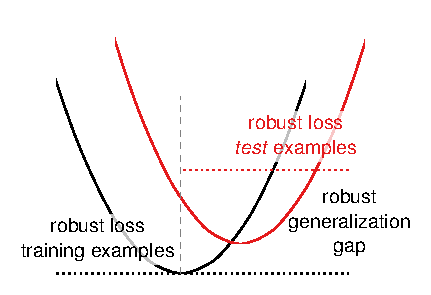
\includegraphics[height=5.75cm,clip,trim={0cm 0cm 0cm 1cm}]{fig/main_illustration2.pdf}
		\end{center}
	\end{frame}
	
	\begin{frame}[t]{\bfseries Contributions: Measuring Robust Flatness}
		\Large
		Flat minima in robust loss improve robust generalization:
		\vspace*{-0.25cm}
		
		\begin{center}
			\begin{tikzpicture}
				\clip (0,0) rectangle (11cm,3.49cm);
				\node[above right,inner sep=0pt] at (0,0) {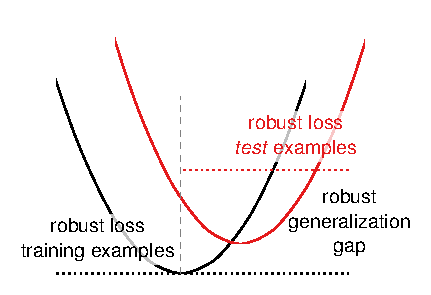
\includegraphics[height=5.75cm,clip,trim={0cm 0cm 0cm 1cm}]{fig/main_illustration2.pdf}};
				\fill[white,path fading=south]
				  (0,0) rectangle (11cm,3.5cm);
			\end{tikzpicture}
		\end{center}
		
		\vspace*{-0.5cm}
		\underline{Contributions:}
		\begin{itemize}
			\item Scale-invariant flatness measure
			\item Relating robustness to flat minima
		\end{itemize}
	\end{frame}
	
	\begin{frame}[t]{\bfseries Measuring Robust Flatness}
		\Large
		\vspace*{0.15cm}
		\begin{center}
			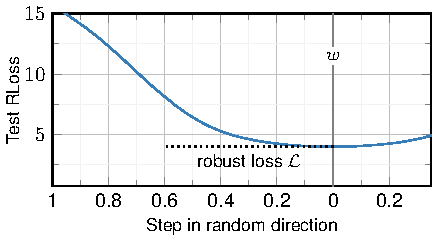
\includegraphics[width=11cm]{fig/main_illustration1.pdf}
		\end{center}
	\end{frame}
	
	\begin{frame}[t]{\bfseries Measuring Robust Flatness}
		\Large
		\vspace*{-0.5cm}
		\begin{center}
			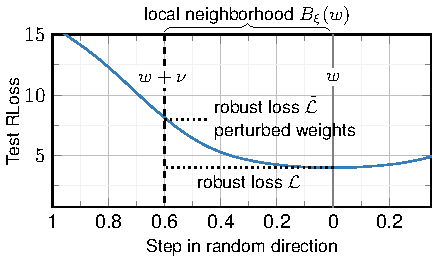
\includegraphics[width=11cm]{fig/main_illustration1_2.pdf}
		\end{center}
	\end{frame}
		
	\begin{frame}[t]{\bfseries Measuring Robust Flatness}
		\Large
		\vspace*{-0.5cm}
		\begin{center}
			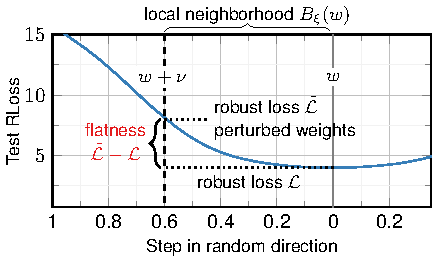
\includegraphics[width=11cm]{fig/main_illustration1_3.pdf}
		\end{center}
	\end{frame}
	
	\begin{frame}[t]{\bfseries Measuring Robust Flatness}
		\Large
		\vspace*{-0.5cm}
		\begin{center}
			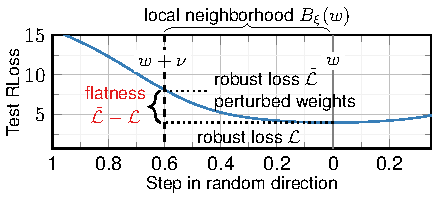
\includegraphics[width=9cm]{fig/main_illustration1_4.pdf}
		\end{center}
		\vspace*{-0.25cm}
		Robust flatness:
		\begin{align}
			\tilde{\mathcal{L}} - \mathcal{L} = \mathbb{E}_{\nu \in B_\xi(w)}[\max\limits_{\|\delta\|_\infty \leq \epsilon} \mathcal{L}(f(x{+}\delta; w{+}\nu), y)] - \max\limits_{\|\delta\|_\infty \leq \epsilon} \mathcal{L}(f(x{+}\delta;w), y)\notag
		\end{align}
	\end{frame}
	
	\begin{frame}[t]{\bfseries Measuring Robust Flatness}
		\Large
		\vspace*{-0.5cm}
		\begin{center}
			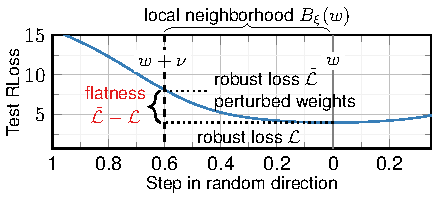
\includegraphics[width=9cm]{fig/main_illustration1_4.pdf}
		\end{center}
		\vspace*{-0.25cm}
		\emph{Scale-invariant} neighborhood in weight space:
		\begin{align}
			B_\xi(w) = \{w + \nu : {\color{MPIIred}\|\nu^{(l)}\|_2 \leq \xi \|w^{(l)}\|_2} \forall\text{ layers }l\}\notag
		\end{align}
	\end{frame}
	
	\begin{frame}[t]{\bfseries Robust Flatness and Overfitting}
		\Large
		Robust overfitting leads to sharper minima:
		
		\centering
		\vspace*{8px}
		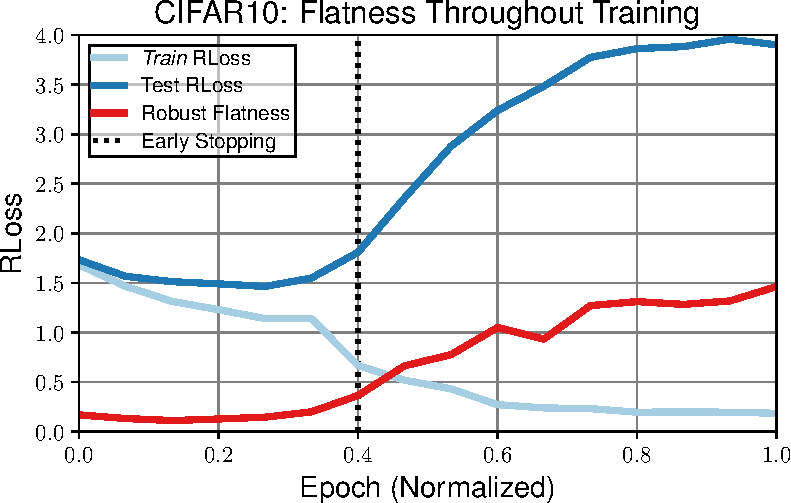
\includegraphics[height=5.5cm]{plots/talk_overview2.pdf}
	\end{frame}
	
	\begin{frame}[t]{\bfseries Robust Flatness and Overfitting}
		\Large
		Robust overfitting leads to sharper minima:
		
		\centering
		\vspace*{6px}
		\begin{minipage}[t]{0.425\textwidth}
			\begin{tikzpicture}[remember picture]\node[opacity=0.5] at (0,0) {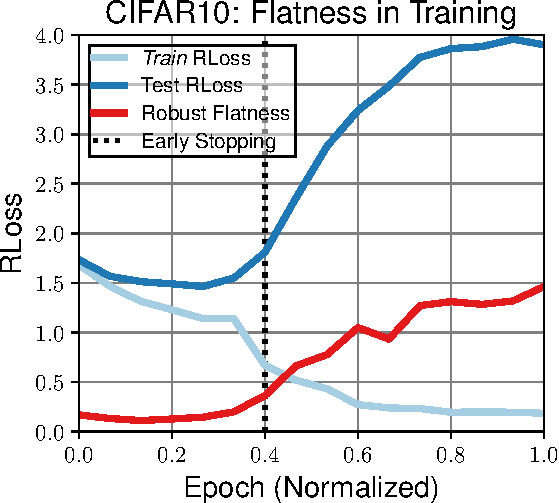
\includegraphics[height=5.5cm]{plots/talk_overview22.pdf}};\end{tikzpicture}
		\end{minipage}
		\begin{minipage}[t]{0.09\textwidth}
			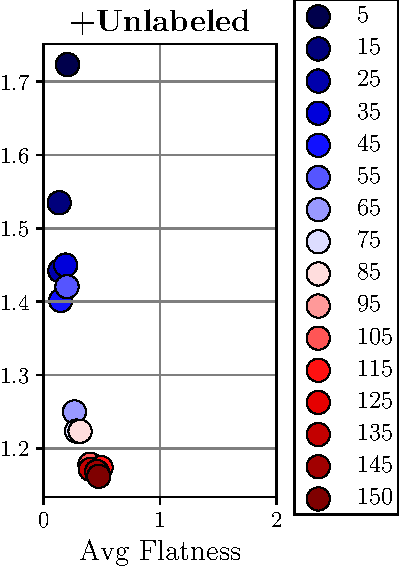
\includegraphics[height=5.5cm,clip,trim={5cm 0cm 0cm 0cm}]{../paper/plots_main_flatness_epochs_correlation_seq_500k}
		\end{minipage}
		\begin{minipage}[t]{0.275\textwidth}
			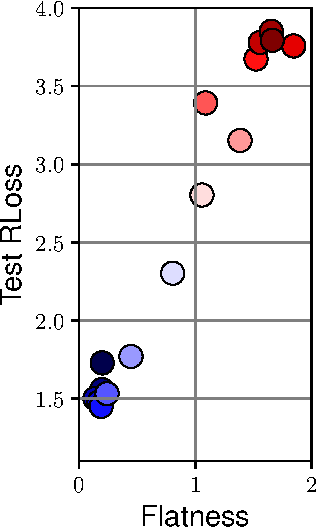
\includegraphics[height=5.5cm]{plots/talk_flatness_epochs_correlation_seq2.pdf}
		\end{minipage}
	\end{frame}
	
	\begin{frame}[t]{\bfseries Robust Overfitting and Regularization}
		\Large
		\centering
		\begin{minipage}[t]{0.075\textwidth}
			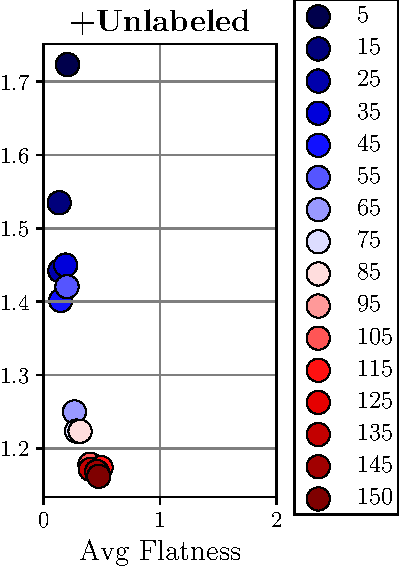
\includegraphics[height=5.5cm,clip,trim={5cm 0cm 0cm 0cm}]{../paper/plots_main_flatness_epochs_correlation_seq_500k}
		\end{minipage}
		\begin{minipage}[t]{0.225\textwidth}
			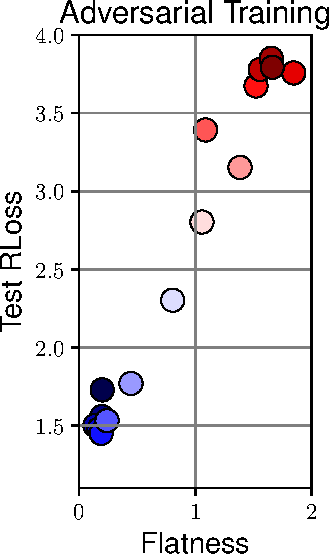
\includegraphics[height=5.5cm]{plots/talk_flatness_epochs_correlation_seq.pdf}
		\end{minipage}
		\begin{minipage}[t]{0.2\textwidth}
			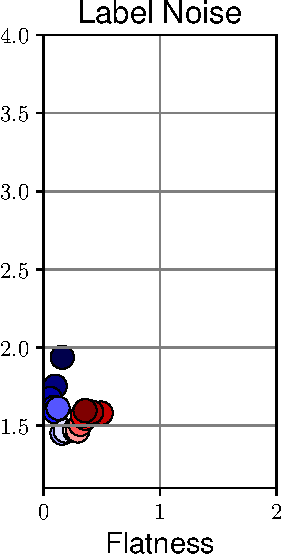
\includegraphics[height=5.5cm]{plots/talk_flatness_epochs_correlation_seq_ln.pdf}
		\end{minipage}
		\begin{minipage}[t]{0.2\textwidth}
			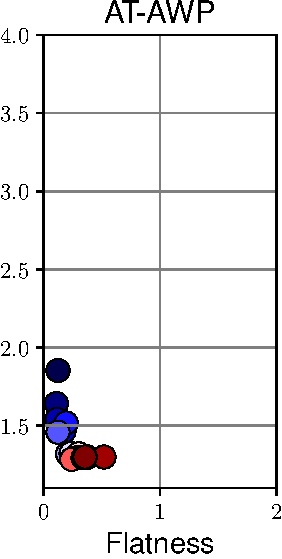
\includegraphics[height=5.5cm]{plots/talk_flatness_epochs_correlation_seq_awp.pdf}
		\end{minipage}
		\begin{minipage}[t]{0.2\textwidth}
			\hphantom{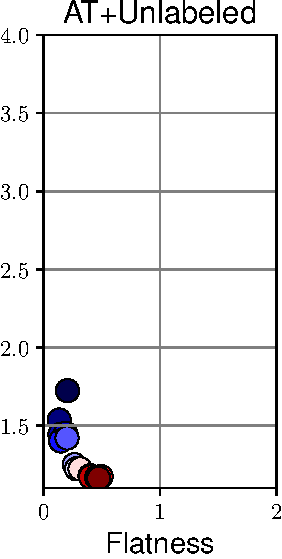
\includegraphics[height=5.5cm]{plots/talk_flatness_epochs_correlation_seq_500k.pdf}}
		\end{minipage}
	\end{frame}
	
	\begin{frame}[t]{\bfseries Robust Overfitting and Regularization}
		\Large
		\centering
		\begin{minipage}[t]{0.075\textwidth}
			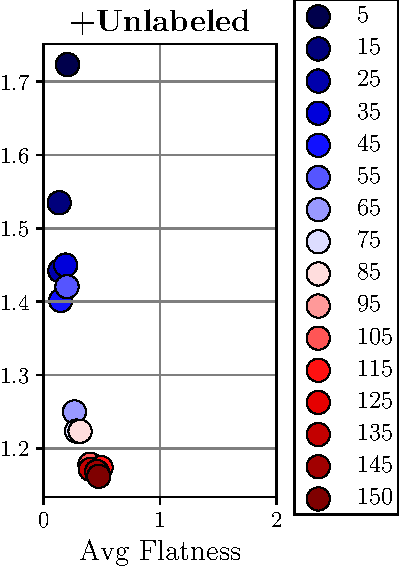
\includegraphics[height=5.5cm,clip,trim={5cm 0cm 0cm 0cm}]{../paper/plots_main_flatness_epochs_correlation_seq_500k}
		\end{minipage}
		\begin{minipage}[t]{0.225\textwidth}
			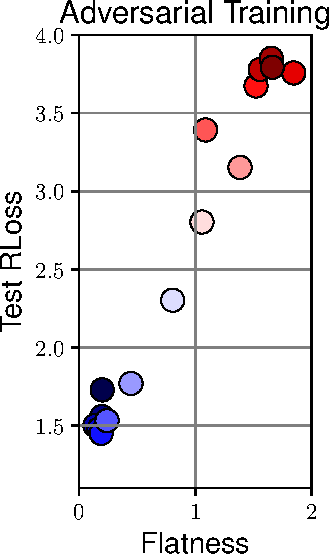
\includegraphics[height=5.5cm]{plots/talk_flatness_epochs_correlation_seq.pdf}
		\end{minipage}
		\begin{minipage}[t]{0.2\textwidth}
			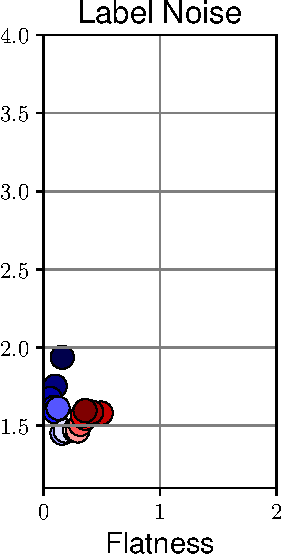
\includegraphics[height=5.5cm]{plots/talk_flatness_epochs_correlation_seq_ln.pdf}
		\end{minipage}
		\begin{minipage}[t]{0.2\textwidth}
			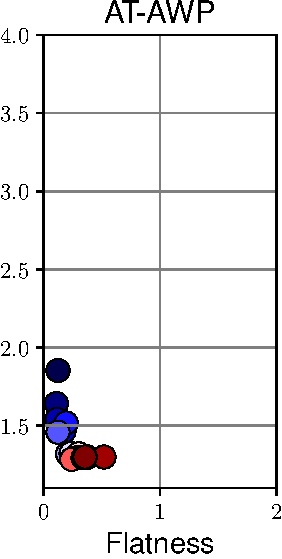
\includegraphics[height=5.5cm]{plots/talk_flatness_epochs_correlation_seq_awp.pdf}
		\end{minipage}
		\begin{minipage}[t]{0.2\textwidth}
			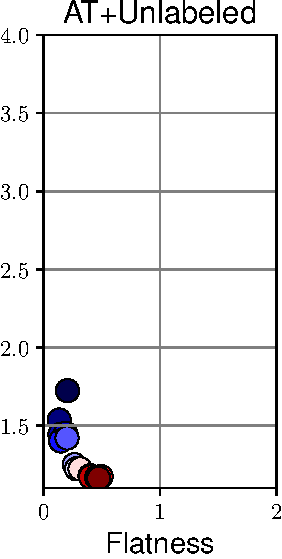
\includegraphics[height=5.5cm]{plots/talk_flatness_epochs_correlation_seq_500k.pdf}
		\end{minipage}
		\begin{tikzpicture}[remember picture,overlay]
			\node[anchor=west,MPIIred,fill=white,text opacity=1,draw opacity=1,fill opacity=0.5,inner sep=1pt] at (-10.25,4){\small \begin{tabular}{@{}c@{}}RErr\\62.8\%\end{tabular}};
			\node[anchor=west,MPIIred,fill=white,text opacity=1,draw opacity=1,fill opacity=0.5,inner sep=1pt] at (-8,1.25){\small \begin{tabular}{@{}c@{}}RErr\\56.2\%\end{tabular}};
			\node[anchor=west,MPIIred,fill=white,text opacity=1,draw opacity=1,fill opacity=0.5,inner sep=1pt] at (-5,1){\small \begin{tabular}{@{}c@{}}RErr\\54.3\%\end{tabular}};
			\node[anchor=west,MPIIred,fill=white,text opacity=1,draw opacity=1,fill opacity=0.5,inner sep=1pt] at (-1.9,0.75){\small \begin{tabular}{@{}c@{}}RErr\\48.9\%\end{tabular}};
		\end{tikzpicture}
	\end{frame}
	
	\begin{frame}{\bfseries Robust Flatness and Hyper-Parameters}
		\Large
		\vspace*{-0.25cm}
		\centering
		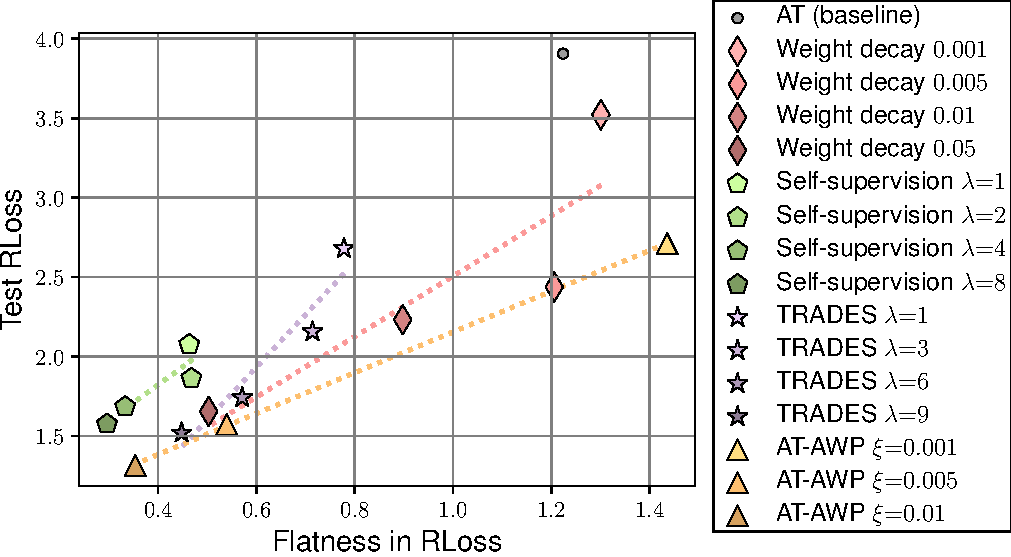
\includegraphics[width=11.5cm]{plots/talk_flatness_methods.pdf}
	\end{frame}
	
	\begin{frame}{\bfseries Robust Flatness \& Robust Generalization}
		\Large
		\centering
		\vspace*{-0.25cm}
		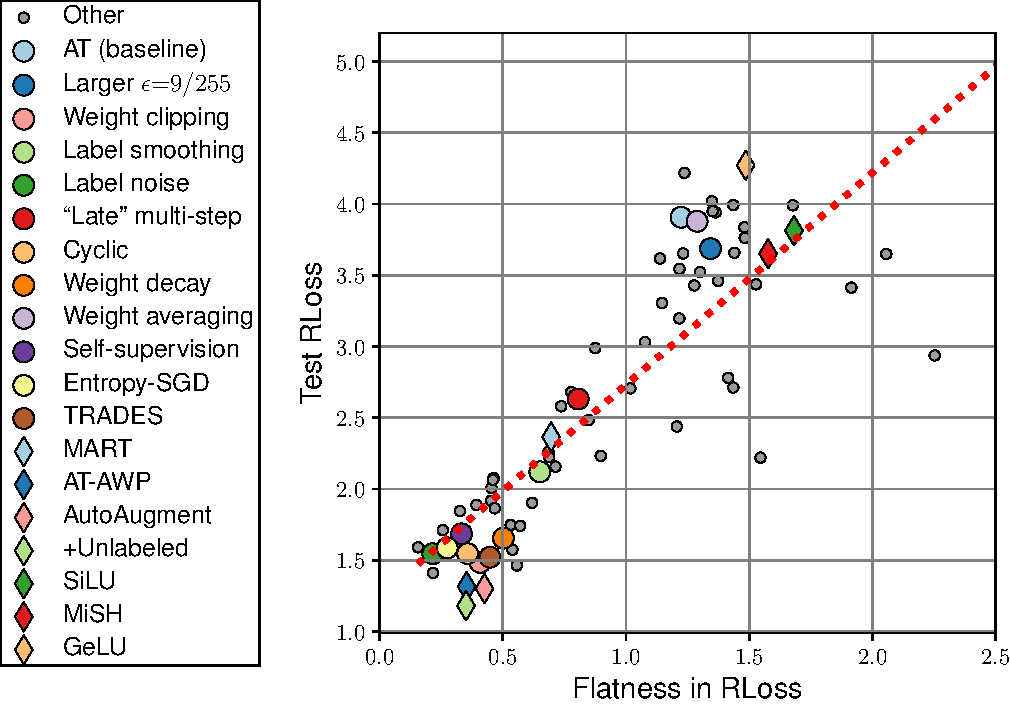
\includegraphics[height=6.35cm]{plots/talk_flatness_correlation_seq_loss2.pdf}
	\end{frame}
	
	\begin{frame}{\bfseries Robust Flatness \& Robust Generalization}
		\Large
		\centering
		\vspace*{-0.25cm}
		\includegraphics[height=6.35cm]{plots/talk_flatness_seq_test_train.pdf}
		\includegraphics[height=6.35cm]{plots/talk_flatness_correlation_seq_last_best_loss.pdf}
	\end{frame}
	
	\begin{frame}[t]{\bfseries Conclusion: Flatness and Robustness}
		\Large
		\vspace*{-0.25cm}
		\begin{itemize}
			\item Robust overfitting caused by sharp minima
			\item Robust flatness correlates with robust generalization
		\end{itemize}
		
		\begin{center}
			\includegraphics[width=10cm]{plots/talk_flatness_correlation_seq_loss3.pdf}
		\end{center}
		\vspace*{-0.15cm}
		\begin{tcolorbox}[
			enhanced,
			boxsep=4pt,
			left=0pt,
			right=0pt,
			top=2pt,
			toptitle=0pt,
			bottomtitle=2pt,
			bottom=0pt,
			colback=gray!12!white,
			colframe=gray!12!white,
			width=1\textwidth, 
			enlarge left by=0mm,
			arc=0pt,outer arc=0pt,
			boxrule=1pt,
			title=,%\bfseries More details:,
			coltitle=MPIIblack,
			colbacktitle=gray!12!white,
			titlerule style=white,
			collower=MPIIblack,
			]
			\color{MPIIblack}
			\textbf{Paper} \& more: \href{http://davidstutz.de/flatness}{\texttt{davidstutz.de/flatness}}
		\end{tcolorbox}
	\end{frame}
\end{document}
